\documentclass{report}
\usepackage[polish]{babel}
\usepackage[utf8]{inputenc}
\usepackage{indentfirst}
\usepackage[T1]{fontenc}
\usepackage{graphicx} 
\usepackage{listings}
\usepackage{xcolor}
\lstset { %
    language=C++,
    backgroundcolor=\color{black!5}, % set backgroundcolor
    basicstyle=\footnotesize,% basic font setting
}
\title{Ciąg Fibonacciego}
\author{Marcin Seferyn}
\date{12.12.2019}
\begin{document}
\maketitle
\newpage
\tableofcontents
\newpage
\chapter{Wstęp}
\section{Kim był Leonardo Fibonacci}
\cite{fib}
Leonardo z Pizy, urodzony ok. 1175 roku w Pizie - zmarł w 1250 roku. Był włoskim matematykiem, znany jako Leonardo Fibonaccim, Filius Bonacci oraz Leonardo Pisano
\subsection{Życiorys}
\cite{fib2}
Jego ojciec, Guglielmo z rodziny Bonacci, zajmował stanowisko dyplomatyczne w Afryce północnej i Fibonacci tam właśnie się kształcił. Pierwsze lekcje matematyki pobierał od arabskiego nauczyciela w mieście Boużia (dziś algierska Bidżaja). Dużo podróżował najpierw razem z ojcem, później samodzielnie, odwiedzając i kształcąc się w takich miejscach jak Egipt, Syria, Prowansja, Grecja i Sycylia. W czasie swych podróży po Europie i po krajach Wschodu miał okazję poznać osiągnięcia matematyków arabskich i hinduskich, między innymi dziesiętny system liczbowy.
Około 1200 roku Fibonacci zakończył podróże i powrócił do Pizy.
Tam zajął się opracowywaniem wielu zagadnień starożytnej matematyki. Żył w epoce przed wynalezieniem druku, dlatego jego dzieła mogły zostać rozpowszechnione jedynie za pomocą ręcznego odpisu. Z tego powodu do dziś przetrwało jedynie kilka z jego prac.
Fibonacci zasłużył się dla rozwoju miasta. Jego wysiłki zostały docenione przez cesarza Fryderyka II. Zmarł w Pizie w 1250 roku.


\begin{figure}[h]
\center
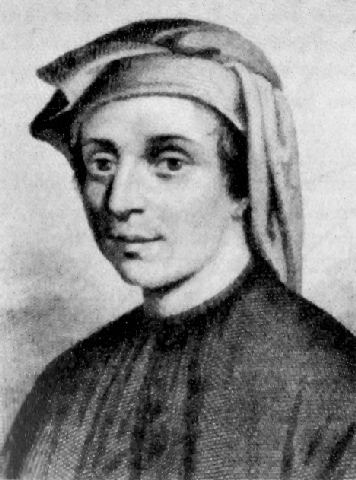
\includegraphics[scale=0.6]{fibo}
\caption{Leonardo Fibonacci}
\end{figure}
\newpage
\section{Dokonania}
\cite{fib3}
\textbf{Fibonacci} był niezwykle utalentowanym matematykiem, jednak wiele z jego prac i teorii nie oddziałało na rozwój matematyki, ponieważ pozostały w dużej mierze nieznane w okresie średniowiecza.
Jednym z ważniejszych dzieł Leonarda z Pizy było \textit{Liber abaci}, które stanowiło wykład azjatyckich osiągnięć w dziedzinie matematyki. Pojawiły się tu takie pojęcia jak: liczby ujemne, zero, pozycyjny system zapisu liczby, równania liniowe i kwadratowe.
Ponadto ważną pracą była \textit{Practica geometriae}, gdzie Fibonacci po raz pierwszy użył algebry w dziedzinie geometrii.
\subsection{Liber Abaci}
\cite{fib4}
\textbf{Liber abaci} lub \textbf{Liber abbaci} – księga matematyczna z 1202, dotycząca arytmetyki. Jej tytuł tłumaczony jest współcześnie jako Księga liczydła lub Księga rachunków. Liber Abaci była jedną z pierwszych zachodnich książek, które opisywały hindusko-arabski system liczbowy i używały symboli tradycyjnie określanych jako „cyfry arabskie”. Uwzględniając zastosowania zarówno dla komercyjnych handlowców, jak i matematyków, przyczyniło się to do przekonania opinii publicznej o wyższości tego systemu i wykorzystaniu go.
\begin{figure}[h]
\center
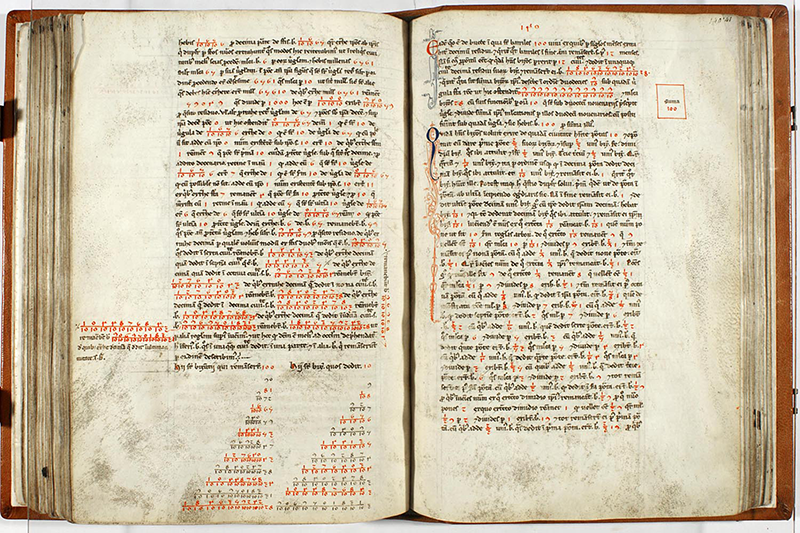
\includegraphics[scale=2]{liberabaci3}
\caption{Liber Abaci}
\end{figure}
\newpage
\chapter{Ciąg Fibonacciego}
\section {Czym jest ciąg Fibonacciego}
\cite{fib5}
\textbf{Ciąg Fibonacciego} – ciąg liczb naturalnych określony rekurencyjnie w sposób następujący:
Pierwszy wyraz jest równy 0, drugi jest równy 1, każdy następny jest sumą dwóch poprzednich. 
\newline
\textbf{Formalnie:}
\newline
\newline
$
\Large{F_{n} = \left\{ \begin{array}{ll}
0 & \textrm{dla $n>0$}\\
1 & \textrm{dla $n=1$}\\
F_{n-1} + F_{n-2} & \textrm{dla $ n > 1 $}
\end{array} \right. }
$
\newline
\begin{center}

\LARGE{\textbf{Pierwsze 11 elementów ciągu}
  \begin{tabular}{ | c | c | c | c | c | c | c | c | c | c | c |}
    \hline
    F_{0} & F_{1} & F_{2} & F_{3} & F_{4} & F_{5} & F_{6} & F_{7} & F_{8} & F_{9} & F_{10}   \\ \hline
    0 & 1 & 1 & 2 & 3 & 5 & 8 & 13 & 21 & 34 & 55 \\ \hline

    
  \end{tabular}
  }
\end{center}}
\newpage
\section{Ciąg Fibonacciego w C++}
\subsection{Iteracyjnie}
\begin{lstlisting}
#include<iostream>
#include<cstdlib>
using namespace std;

void fibonacci(int n)
{    
     long long a = 0, b = 1;
     for(int i=0;i<n;i++)
     {
            cout<<b<<" ";
            b += a;  
            a = b-a;  
     }     
}

int main()
{
    int n;
    cout<<"Podaj ile chcesz wypisac wyrazow ciagu fibonacciego: ";
    cin>>n;
    fibonacci(n);
    system("pause");
    return 0;
}
\end{lstlisting}
\subsection{Rekurencyjnie}
\begin{lstlisting}
#include<iostream>
#include<cstdlib>
using namespace std;

int fib(int n)
{
	if(n<3)
		return 1;
	return fib(n-2)+fib(n-1);
}
int main()
{
	int n;
	cout<<"Podaj nr wyrazu ciagu: ";
	cin>>n;
	cout<<n<<" wyraz ciagu ma wartos "<<fib(n)<<endl;
	system("pause");
	return 0;
}
\end{lstlisting}
\newpage
\begin{thebibliography}{9}
\bibitem{fib} Kim był Fibonacci https://pl.wikipedia.org/wiki/Fibonacci
\bibitem{fib2} Życiorys https://eszkola.pl/matematyka/leonardo-fibonacci-4869.html
\bibitem{fib3} Dokonania https://eszkola.pl/matematyka/leonardo-fibonacci-4869.html
\bibitem{fib4} Liber Abaci https://en.wikipedia.org/wiki/Liber-Abaci
\bibitem{fib5} Ciąg Fibonacciego https://pl.wikipedia.org/wiki/Ciag-Fibonacciego

\end{thebibliography}
\listoffigures

\end{document}
	